\documentclass{beamer}
\usepackage[utf8]{inputenc}
\usepackage[T1]{fontenc}
\usepackage[croatian]{babel}
\usetheme{metropolis}
\usepackage{siunitx}
\usepackage{amsmath}
\usepackage{listings}
\usepackage{verbatim}
\usepackage[makeroom]{cancel}
\usepackage{subcaption}


\title{Analiza rješavanja i rješavanje igre Minesweeper}
\date{\today}
\author{Darko Janeković, Jelena Nemčić}
\institute{Fakultet elektrotehnike i računarstva}
\begin{document}
    \maketitle

    \begin{frame}[t]
        \frametitle{Opis igre}
        \begin{itemize}
            \item<1-> Otvoriti polje
            \item<2-> Označiti ili maknuti oznaku s polja
        \end{itemize}
        \begin{figure}
            \centering
            \visible<1->{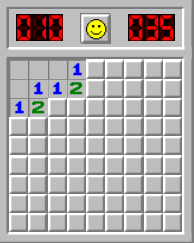
\includegraphics[width=0.4\textwidth]{images/open.png}}
            \visible<2>{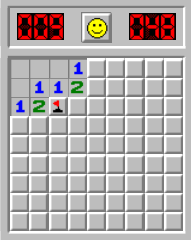
\includegraphics[width=0.4\textwidth]{images/mark.png}}
        \end{figure}
    \end{frame}

    \begin{frame}[t]
        \frametitle{Model problema}

        \begin{table}[ht]
            \centering
            \begin{tabular}{llll}
                                   & 1                      & 2                      & 3                      \\ \cline{2-4}
            \multicolumn{1}{l|}{1} & \multicolumn{1}{l|}{}  & \multicolumn{1}{l|}{}  & \multicolumn{1}{l|}{}  \\ \cline{2-4}
            \multicolumn{1}{l|}{2} & \multicolumn{1}{l|}{1} & \multicolumn{1}{l|}{1} & \multicolumn{1}{l|}{1} \\ \cline{2-4}
            \multicolumn{1}{l|}{3} & \multicolumn{1}{l|}{0} & \multicolumn{1}{l|}{0} & \multicolumn{1}{l|}{0}  \\ \cline{2-4}
            \end{tabular}
        \end{table}

        \begin{itemize}
            \item<1-> $m_{i, j} \in {\bot, \top}$
            \item<2-> Susjedstvo polja $m_{i, j}$: $\mathcal{N}(m_{i, j})$
            \item<3-> Broj mina u susjedstvu polja $m_{i, j}$: $n$.
        \end{itemize}

        \visible<4>{
            \begin{equation}
                \sum_{a \in \mathcal{N}(m_{i, j})} a = n
            \end{equation}
        }
    \end{frame}

    \begin{frame}[t]
        \frametitle{Model problema (2)}

        \begin{table}[ht]
            \centering
            \begin{tabular}{llll}
                                   & 1                      & 2                      & 3                      \\ \cline{2-4}
            \multicolumn{1}{l|}{1} & \multicolumn{1}{l|}{}  & \multicolumn{1}{l|}{}  & \multicolumn{1}{l|}{}  \\ \cline{2-4}
            \multicolumn{1}{l|}{2} & \multicolumn{1}{l|}{1} & \multicolumn{1}{l|}{1} & \multicolumn{1}{l|}{1} \\ \cline{2-4}
            \multicolumn{1}{l|}{3} & \multicolumn{1}{l|}{0} & \multicolumn{1}{l|}{0} & \multicolumn{1}{l|}{0}  \\ \cline{2-4}
            \end{tabular}
        \end{table}

        \begin{align*}
            m_{1, 1} + m_{1, 2} = 1 \\
            m_{1, 1} + m_{1, 2} + m_{1, 3} = 1 \\
            m_{1, 2} + m_{1, 3} = 1 \\
        \end{align*}

        \visible<2->{Rješavanje problema kao problem zadovoljivosti (SAT) ili kao problem programiranja s ograničenjima.}
    \end{frame}

    \begin{frame}[t]
        \frametitle{SAT algoritam - problem zadovoljivosti}

        \begin{table}[ht]
            \centering
            \begin{tabular}{llll}
                                   & 1                      & 2                      & 3                      \\ \cline{2-4}
            \multicolumn{1}{l|}{1} & \multicolumn{1}{l|}{}  & \multicolumn{1}{l|}{}  & \multicolumn{1}{l|}{}  \\ \cline{2-4}
            \multicolumn{1}{l|}{2} & \multicolumn{1}{l|}{1} & \multicolumn{1}{l|}{1} & \multicolumn{1}{l|}{1} \\ \cline{2-4}
            \multicolumn{1}{l|}{3} & \multicolumn{1}{l|}{0} & \multicolumn{1}{l|}{0} & \multicolumn{1}{l|}{0}  \\ \cline{2-4}
            \end{tabular}
        \end{table}

        \visible<1->{Svođenje problema na oblik konjugirane normalne forme (CNF).}
        \begin{multline*}
            \onslide<2->{(m_{1, 1} \vee m_{1, 2}) \wedge (\neg m_{1, 1} \vee \neg m_{1, 2}) \\}
            \onslide<3->{(m_{1, 1} \vee m_{1, 2} \vee m_{1, 3}) \wedge (\neg m_{1, 1} \vee \neg m_{1, 2}) \wedge \nonumber (\neg m_{1, 2} \vee \neg m_{1, 3}) \wedge (\neg m_{1, 3} \vee \neg m_{1, 1}) \\}
            \onslide<4->{(m_{1, 2} \vee m_{1, 3}) \wedge (\neg m_{1, 2} \vee \neg m_{1, 3}) \\}
        \end{multline*}

        \visible<5->{Zaključivanje teoremom dedukcije: $(\Gamma \wedge \neg m_{1, 2})$}

    \end{frame}

    \begin{frame}[t]
        \frametitle{Simpleks algoritam - programiranje s ograničenjima}

        \begin{table}[ht]
            \centering
            \begin{tabular}{llll}
                                   & 1                      & 2                      & 3                      \\ \cline{2-4}
            \multicolumn{1}{l|}{1} & \multicolumn{1}{l|}{}  & \multicolumn{1}{l|}{}  & \multicolumn{1}{l|}{}  \\ \cline{2-4}
            \multicolumn{1}{l|}{2} & \multicolumn{1}{l|}{1} & \multicolumn{1}{l|}{1} & \multicolumn{1}{l|}{1} \\ \cline{2-4}
            \multicolumn{1}{l|}{3} & \multicolumn{1}{l|}{0} & \multicolumn{1}{l|}{0} & \multicolumn{1}{l|}{0}  \\ \cline{2-4}
            \end{tabular}
        \end{table}

        \visible<1->{Metoda rješavanja problema u lineranom programiranju.}
         
        \visible<3->{Simpleks algoritam pronalazi osnovno zadovoljivo rješenje (BFS).}

        \visible<2->{
        \begin{gather*}
            1 \ge m_{i, i} \ge 0 \\
            m_{1, 1} + m_{1, 2} = 1 \\
            m_{1, 1} + m_{1, 2}+ m_{1, 3} = 1 \\
            m_{1, 2} + m_{1, 3} = 1
        \end{gather*}}
    \end{frame}

        \begin{frame}[t]
        \frametitle{Implementacija}
        
         \begin{figure}
            \centering
            \visible<1->{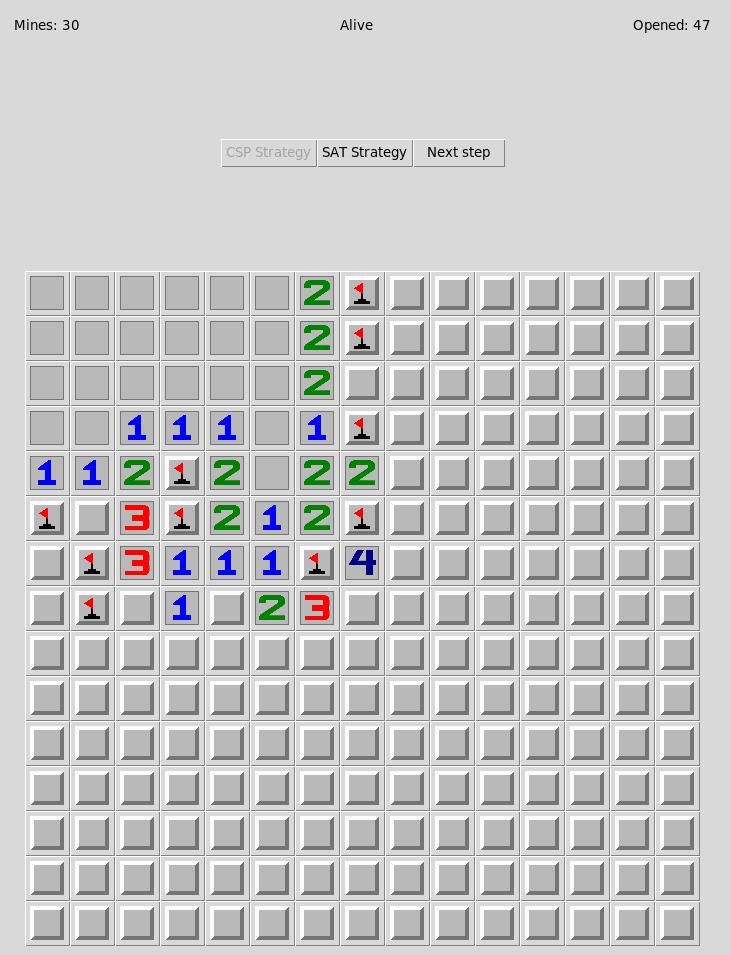
\includegraphics[width=0.4\textwidth]{images/gui.png}}
        \end{figure}

      \begin{itemize}
            \item<2-> Ploča koja sadrži polja i komunicira s grafičkim sučeljem
            \item<3-> Strategija SAT zaključivanja $\rightarrow$ biblioteka \textit{PySAT}
            \item<4-> Simpleks metoda $\rightarrow$ biblioteka \textit{Cassowary}
        \end{itemize}
    \end{frame}
    
      \begin{frame}[t]
        \frametitle{Implementacija}
        
         \begin{figure}
            \centering
            \visible<1->{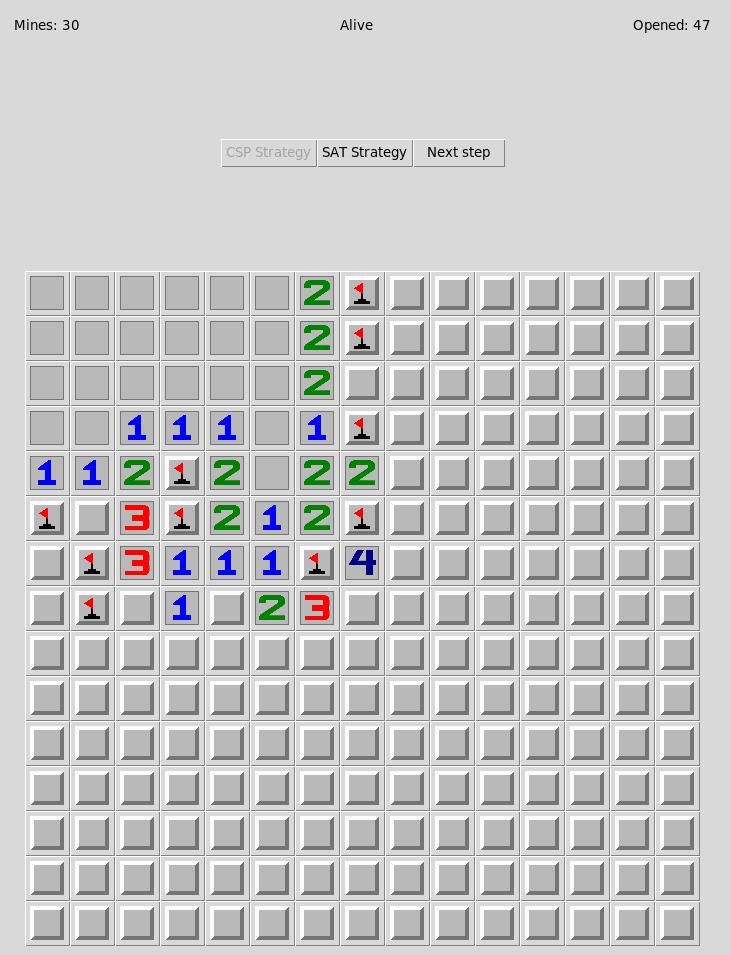
\includegraphics[width=0.4\textwidth]{images/gui.png}}
        \end{figure}

      \begin{itemize}
            \item<2-> Mogućnost odabira strategije
            \item<3-> Praćenje igre potez po potez
            \item<4-> Brojač preostalih mina i otvorenih polja
        \end{itemize}
    \end{frame}

    \begin{frame}[standout]
        Demonstracija i hvala na pažnji!
    \end{frame}
\end{document}
